\begin{pastexam}[label={px:ntut-111-ci-03}]{北科大資工所 111 學年度 第四題}
（簡答）

(15 pts) Please answer the following questions concisely. You do not need to provide the details.
\begin{enumerate}[label=(\arabic*)]
\item Find the asymptotic upper bound (using Big-O notation) for $T(n) = 3T(n-1) + 2$ with $T(0) = 1$. (3 pts)
\item Let $B$ be a binomial tree of size 29. Please draw the shape of this binomial tree.(3 pts)
\item Please write the following infix expression in postfix form: (3 pts)\\
$((2\times(4-1))-(3+1))+((6/3)\times(2+4))$.
\item Suppose that we have a complete binary tree represented by the following array, where each cell of the array contains a key value. Please draw this complete binary tree. (3 pts)
\begin{center}
\begin{tabular}{|c|c|c|c|c|c|c|c|c|c|c|}\hline
Index & 1 & 2 & 3 & 4 & 5 & 6 & 7 & 8 & 9 & 10\\\hline
Key & 3 & 12 & 44 & 30 & 20 & 25 & 55 & 87 & 16 & 27\\\hline
\end{tabular}
\end{center}
\item A $k$-ary tree is a tree of which each node has at most $k$ children. What is the maximum number of nodes in a $k$-ary tree of height $h$? (3 pts)
\end{enumerate}
\end{pastexam}

\begin{pastsoln}
答案：(1) $O(3^n)$（精確值 $T(n) = 2 \cdot 3^n - 1$）；(2) 見下圖，是 $B_4, B_3, B_2, B_0$ 四棵二項樹；
(3) \texttt{2 4 1 - * 3 1 + - 6 3 / 2 4 + * +}；(4) 見下圖；(5) $\frac{k^{h+1} - 1}{k - 1}$（$k \ge 2$，根的深度為 $0$）。

五個小題分屬資結書第~2、8、6、7、7~章；第~7~章佔兩個小題，本題放在第~7~章。 題目說不必寫細節，下面仍把理由寫出來。

\textbf{(1)} 兩邊加 $1$：$T(n) + 1 = 3T(n-1) + 3 = 3\bigl(T(n-1) + 1\bigr)$。 令 $S(n) = T(n) + 1$，$S(0) = 2$，$S(n) = 3S(n-1)$，所以
$S(n) = 2 \cdot 3^n$，$T(n) = 2 \cdot 3^n - 1$（資結書第~2.5~節）。 檢查：$T(1) = 3 + 2 = 5 = 2 \cdot 3 - 1$，$T(2) = 15 + 2 = 17 = 2 \cdot 9 - 1$。
答案 $T(n) = O(3^n)$（其實是 $\Theta(3^n)$）。

\textbf{(2)} 原題有誤：二項樹 $B_k$ 恰有 $2^k$ 個節點，沒有大小為 $29$ 的二項樹。 這裡採用的解讀是「有 $29$ 個節點的二項\textbf{堆積}」
（資結書第~8.5.6~節）。 二項堆積裡每種大小的二項樹最多一棵，各棵的大小對應節點數的二進位表示：$29 = 11101_2 = 16 + 8 + 4 + 1$，
所以由 $B_4$（$16$ 個）、$B_3$（$8$ 個）、$B_2$（$4$ 個）、$B_0$（$1$ 個）四棵組成，形狀唯一。 $B_k$ 的根有 $k$ 個子節點，由左到右
是 $B_{k-1}, \ldots, B_1, B_0$：
\begin{center}
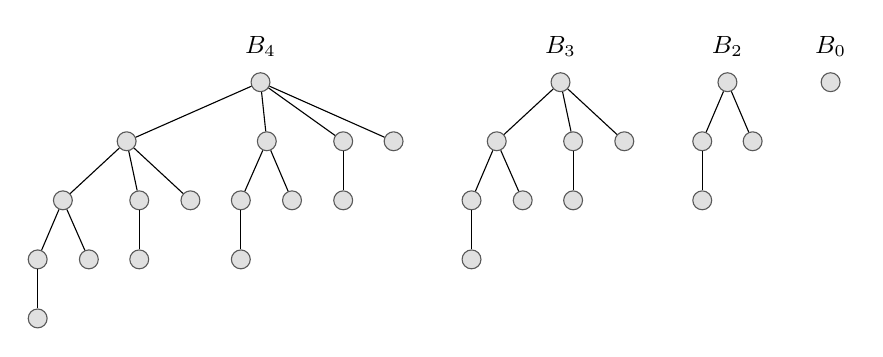
\begin{tikzpicture}[b/.style={circle,draw=black!65,fill=black!12,minimum size=2.4mm,inner sep=0pt}]
\node[b] (n5) at (0.19,-3.00) {};
\node[b] (n4) at (0.19,-2.25) {};
\draw (n4)--(n5);
\node[b] (n6) at (0.84,-2.25) {};
\node[b] (n3) at (0.51,-1.50) {};
\draw (n3)--(n4);
\draw (n3)--(n6);
\node[b] (n8) at (1.48,-2.25) {};
\node[b] (n7) at (1.48,-1.50) {};
\draw (n7)--(n8);
\node[b] (n9) at (2.13,-1.50) {};
\node[b] (n2) at (1.32,-0.75) {};
\draw (n2)--(n3);
\draw (n2)--(n7);
\draw (n2)--(n9);
\node[b] (n12) at (2.77,-2.25) {};
\node[b] (n11) at (2.77,-1.50) {};
\draw (n11)--(n12);
\node[b] (n13) at (3.42,-1.50) {};
\node[b] (n10) at (3.10,-0.75) {};
\draw (n10)--(n11);
\draw (n10)--(n13);
\node[b] (n15) at (4.07,-1.50) {};
\node[b] (n14) at (4.07,-0.75) {};
\draw (n14)--(n15);
\node[b] (n16) at (4.71,-0.75) {};
\node[b] (n1) at (3.02,0.00) {};
\draw (n1)--(n2);
\draw (n1)--(n10);
\draw (n1)--(n14);
\draw (n1)--(n16);
\node[font=\small,anchor=south] at (3.02,0.2) {$B_4$};
\node[b] (n20) at (5.70,-2.25) {};
\node[b] (n19) at (5.70,-1.50) {};
\draw (n19)--(n20);
\node[b] (n21) at (6.35,-1.50) {};
\node[b] (n18) at (6.02,-0.75) {};
\draw (n18)--(n19);
\draw (n18)--(n21);
\node[b] (n23) at (6.99,-1.50) {};
\node[b] (n22) at (6.99,-0.75) {};
\draw (n22)--(n23);
\node[b] (n24) at (7.64,-0.75) {};
\node[b] (n17) at (6.83,0.00) {};
\draw (n17)--(n18);
\draw (n17)--(n22);
\draw (n17)--(n24);
\node[font=\small,anchor=south] at (6.83,0.2) {$B_3$};
\node[b] (n27) at (8.63,-1.50) {};
\node[b] (n26) at (8.63,-0.75) {};
\draw (n26)--(n27);
\node[b] (n28) at (9.27,-0.75) {};
\node[b] (n25) at (8.95,0.00) {};
\draw (n25)--(n26);
\draw (n25)--(n28);
\node[font=\small,anchor=south] at (8.95,0.2) {$B_2$};
\node[b] (n29) at (10.26,0.00) {};
\node[font=\small,anchor=south] at (10.26,0.2) {$B_0$};
\end{tikzpicture}
\end{center}
共 $16 + 8 + 4 + 1 = 29$ 個節點，最高的 $B_4$ 高度是 $4$。

\textbf{(3)} 先找出每個運算子的兩個運算元（括號已經寫明順序），再改成「運算元、運算元、運算子」（資結書第~6.3.3~節）：
\begin{itemize}
\item $2 \times (4 - 1)$ $\to$ \texttt{2 4 1 - *}；$3 + 1$ $\to$ \texttt{3 1 +}；兩者相減 $\to$ \texttt{2 4 1 - * 3 1 + -}。
\item $6/3$ $\to$ \texttt{6 3 /}；$2 + 4$ $\to$ \texttt{2 4 +}；兩者相乘 $\to$ \texttt{6 3 / 2 4 + *}。
\item 最外層相加：\texttt{2 4 1 - * 3 1 + - 6 3 / 2 4 + * +}。
\end{itemize}
檢查：用堆疊計算後序式（資結書虛擬碼~6.7），$2 \cdot 3 = 6$，$6 - 4 = 2$，$6/3 = 2$，$2 \cdot 6 = 12$，$2 + 12 = 14$；原式
$(6 - 4) + (2 \times 6) = 14$，相同。

\textbf{(4)} 陣列從 $1$ 開始時，$A[i]$ 的左、右子節點是 $A[2i]$、$A[2i+1]$（資結書第~7.2.1~節）：$3$ 的子節點是 $12, 44$；$12$ 的是
$30, 20$；$44$ 的是 $25, 55$；$30$ 的是 $87, 16$；$20$ 只有左子節點 $27$（$A[10]$）。
\begin{center}
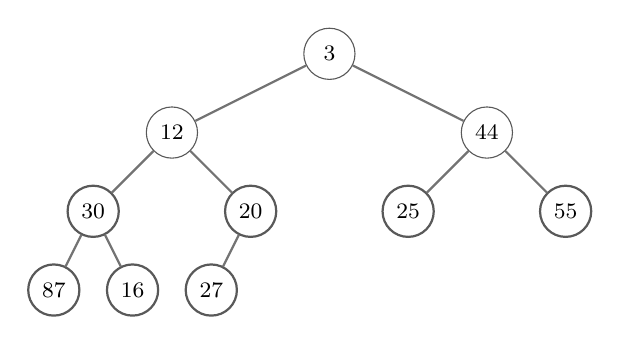
\begin{tikzpicture}[level distance=10mm, edge from parent/.style={draw=black!55, thick},
  every node/.style={circle, draw=black!65, minimum size=6.5mm, inner sep=0pt, font=\footnotesize},
  level 1/.style={sibling distance=40mm}, level 2/.style={sibling distance=20mm}, level 3/.style={sibling distance=10mm}]
\node {3}
  child {node {12}
    child {node {30} child {node {87}} child {node {16}}}
    child {node {20} child {node {27}} child[missing]}}
  child {node {44}
    child {node {25}}
    child {node {55}}};
\end{tikzpicture}
\end{center}
（這只是一棵完全二元樹，不是堆積也不是搜尋樹，例如 $30 > 16$、$12 < 20$ 都不影響。）

\textbf{(5)} 高度 $h$ 指根到最深葉子的邊數（和第二題 (3) 一樣，根在深度 $0$）。 深度 $i$ 最多 $k^i$ 個節點（每個節點最多 $k$ 個子節點，
資結書第~7.1~節），所以最多
\[
\sum_{i=0}^{h} k^i = 1 + k + \cdots + k^h = \frac{k^{h+1} - 1}{k - 1} \qquad (k \ge 2),
\]
每個內部節點都有 $k$ 個子節點、葉子都在深度 $h$ 時達到。 $k = 1$ 時是一條鏈，$h + 1$ 個。 若把高度定義成層數（根算第 $1$ 層），答案改寫成
$\frac{k^h - 1}{k - 1}$。 例如 $k = 2$、$h = 3$：$1 + 2 + 4 + 8 = 15 = 2^4 - 1$。
\end{pastsoln}
